% !TeX program = pdflatex
% Native official Copernicus 7.16 package, GMD single-column manuscript format.
\documentclass[gmd,manuscript]{copernicus}
\usepackage{booktabs}
\begin{document}
\title{State resynchronization in reservoir ensembles without additional observations}
\Author[1]{Soobin}{Choi}
\Author[1][pwkim@unist.ac.kr]{Pilwon}{Kim}
\affil[1]{Department of Mathematical Science, Ulsan National Institute of Science and Technology, Ulsan, Republic of Korea}
\runningtitle{State resynchronization in reservoir ensembles}
\runningauthor{S. Choi and P. Kim}
\received{}
\pubdiscuss{}
\revised{}
\accepted{}
\published{}
\firstpage{1}
\maketitle
\begin{abstract}
Autonomous learned models can depart from the dynamics represented in their training data. We study resynchronization, which drives a selected member's fixed model with another member's generated history before autonomous prediction resumes, without additional observations. We distinguish changes in subsequent member-generated outputs from changes in the returned ensemble. In five 300-member reservoir examples, the method lowers marginal Wasserstein distance for both own and returned outputs and reduces returned-population spread loss relative to no intervention. Continuous ranked probability score improvements are less uniform. Matched next-segment interventions in Duffing and Kuramoto--Sivashinsky show that the additional contribution of history reconstruction beyond boundary-input transfer depends on the setting. These results connect state intervention to population-level outcomes rather than establish universal recovery or climate replication. Supporting analyses examine consistency across additional model banks and physical initial conditions, and the relation between replay length, quality and recorded computation. Joint selection of replay length and intervention parameters remains a question for future policy research.

\end{abstract}
% Generated from shared science; edit originals then regenerate.
\introduction

Chaotic trajectories lose pointwise agreement under small model errors, whereas long-run state distributions can remain predictable. Reservoir computing, particularly echo state networks (ESNs), has been used to approximate autonomous chaotic dynamics \citep{jaeger2004harnessing,pathak2017using,pathak2018model}. Accurate predictions under observational driving do not by themselves establish reliable autonomous behavior \citep{haluszczynski2019good,hart2023attractor,platt2021robust}. A trained model may instead approach a fixed output, develop incorrect recurrences or depart from the observed state distribution.

In the ESNs considered here, only the readout is fitted by regression. Ensembles can therefore combine models with different random recurrent parameters without training those parameters. Reservoir ensembles have been used for uncertainty estimation and climate predictability \citep{mcdermott2019deep,nadiga2021reservoir}, and reservoir surrogates have been combined with data assimilation \citep{tomizawa2021combining,penny2022integrating}. Here the members are model realizations, rather than samples from a specified distribution of physical initial conditions.

We assess ensemble quality through three complementary indicators: marginal Wasserstein distance ($W_1$), spread and the continuous ranked probability score (CRPS). They describe returned-state distributions, simultaneous dispersion and marginal probabilistic quality, respectively \citep{gneiting2007proper,leutbecher2008ensemble}. Diversity and calibration require additional checks \citep{pennell2010number,kuncheva2003measures,gneiting2007calibration}. Distributional agreement also does not establish temporal fidelity \citep{hess2023generalized,koppe2019identifying}. We use ``ensemble health'' only as an operational description of these separate properties. Distance from the population center is a screening criterion, not a diagnosis of physical failure.

Resync drives a recipient's own fixed model with the generated history of a nonselected donor, after which the recipient resumes autonomous prediction. It uses the input-driven state update that also supports observational warm-up and synchronization \citep{pecora1990synchronization,lu2018attractor}. Neither hidden states nor model parameters are copied between members. We call the candidates generated by each model its \emph{own} outputs and the population issued after donor replacement the \emph{returned} outputs. This distinction separates subsequent model behavior from changes to the current output record.

Cross-pollination in time combines model-generated sequences in observation space, reconstructs constituent model states through data assimilation and continues model integration \citep{du2017crosspollination}. Its illustrated pseudo-orbit implementation optimizes model-state sequences; resync instead reconstructs a state through the recipient's fixed input-update map. Supermodeling also exchanges dynamical information among imperfect models \citep{schevenhoven2019supermodels}. The contribution examined here is the connection between generated-history intervention in a recipient's fixed model, its subsequent own autonomous output, and the resulting returned-population quality under truth-free screening.

Our central question is whether generated-history state intervention can restore useful autonomous behavior in a departing recipient, and how the resulting member-level changes affect an ensemble. We examine subsequent own outputs alongside returned-population W1, spread and CRPS. This connects the state intervention to its population consequences without treating member recovery as a guarantee of ensemble improvement. Full climate replication and calibrated physical initial-condition uncertainty are outside the present claim.

Figure~\ref{fig:intuition} describes resync. The main ensemble comparisons use ESNs; a separate Duffing LSTM example illustrates the operation in another recurrent architecture.
\begin{figure}[!htbp]
\centering
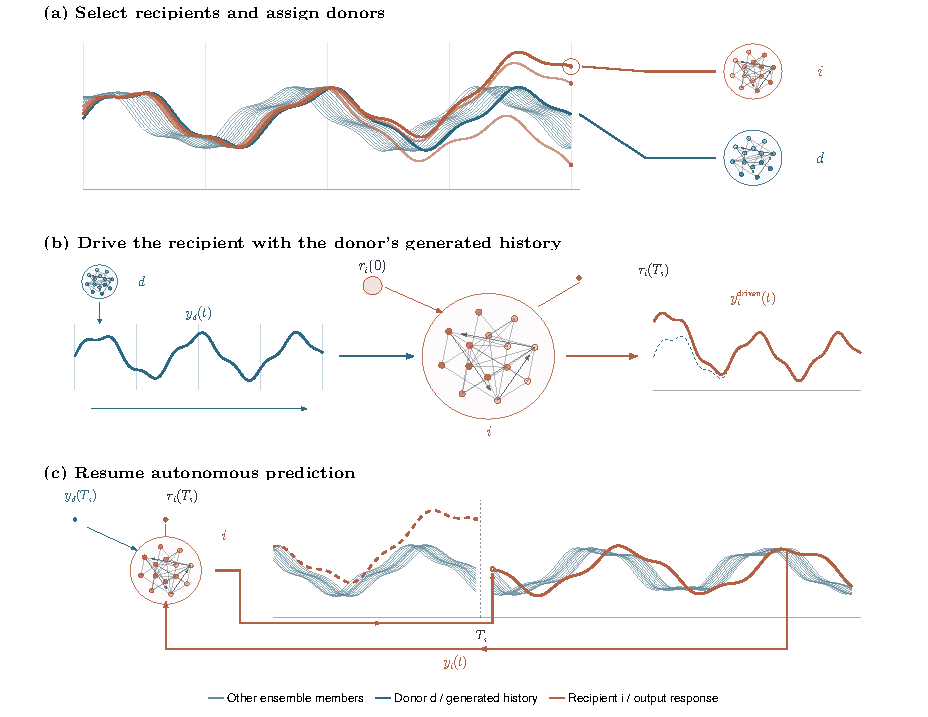
\includegraphics[width=.85\linewidth,height=.68\textheight,keepaspectratio]{figures/fig01.pdf}
\caption{Resynchronization using generated history. \textbf{a,} Select recipient $i$ and nonselected donor $d$. \textbf{b,} Drive the recipient's fixed model with donor outputs, starting from its saved forecast-initialized state $r_i(0)$; the diamond marks the reconstructed state. \textbf{c,} Resume the recipient's autonomous prediction. The original candidate is retained. Curves are schematic, not performance data. Methods specifies the transition to autonomous feedback and the output-record conventions.}
\label{fig:intuition}
\end{figure}



\section{Models and resynchronization procedure}

\subsection{Data, blocks and training settings}
The five systems have 2, 6, 64, 20 and 16 observed variables for Duffing, CDV, KS, QG and Thomas, respectively. QG uses the full two-layer beta-plane channel truncation in \texttt{qgs} v1.0.0 \citep{demaeyer2020qgs}, without dimensionality reduction; Thomas uses a cyclic extension of its three-variable equations. Table~\ref{tab:scheme-design} lists reservoir sizes, training lengths and base intervals. Physical equations, integration steps and complete presets are given in Sect.~\ref{app:note7}.

Training fixes model parameters and normalization. Separate calibration data provide target distributions and empirical references; validation selects scheme parameters; test evaluates the selected scheme. No post-start truth enters online selection or replay. The system-specific base interval $\tau_0$ is fixed before search; interventions occur at $\tau=m\tau_0$, while evaluation durations remain fixed in base units. Sects.~\ref{app:note6}--\ref{app:note7} document data separation, case selection and provenance.

\begin{table}[htbp]
\caption{System dimensions, reservoir sizes, training lengths and base intervals (saved steps). Full presets appear in Sect.~\ref{app:note7}.}\label{tab:scheme-design}
\centering\small\begin{tabular}{lrrrr}\toprule
System & Observed dim. & Reservoir & Training samples & Base $\tau_0$\\\midrule
Duffing & 2 & 200 & 5000 & 600\\
CDV & 6 & 500 & 20000 & 223\\
KS & 64 & 200 & 20000 & 474\\
QG & 20 & 500 & 20000 & 217\\
Thomas & 16 & 400 & 10000 & 100\\
\bottomrule\end{tabular}
\end{table}


Let $u(t)=H(x(t))$, reservoir state $r_i$ and fixed model parameters $\theta_i$. The leaky update and readout are
\begin{align}
r_i(t+1)&=(1-a_i)r_i(t)+a_i\tanh\big(A_i r_i(t)+B_i u(t)+b_i\big),\\
y_i(t+1)&=C_i\phi\big(r_i(t+1)\big).
\end{align}
The readout is fitted by regression. In autonomous prediction each model feeds back its own output. Reservoir seeds represent model realizations rather than samples of physical initial-condition uncertainty.

\subsection{Candidate generation and blind selection}
Candidates are generated over segments of length $\tau$. Per-coordinate mean, population standard deviation, skewness and excess kurtosis form each member's feature vector. Feature standardization and a PCA basis are fitted to length-$\tau$ training windows. The smallest number of components explaining 95\% of training feature variance is retained, with at least two components. Distance from the centroid of finite candidate feature vectors is the blind score. Approximately $pN$ high-scoring members are selected as recipients; nonfinite candidates are explicitly recorded. Donors follow a deterministic cyclic member-index assignment among unselected members (Sect.~\ref{app:note3}). Neither centroid distance nor nonselection establishes physical validity. A nonfinite own candidate remains a recorded failure of that rollout even when subsequent effective-output replacement is finite.

\subsection{Resynchronization and output records}
For the main five-system comparisons, the saved forecast-initialized state $r_i(0)$ is obtained by driving the end-of-training state with up to 1000 observed samples preceding forecast start. These inputs end at $u(-1)$; the first rollout input $u(0)$ is not consumed during this synchronization, and the first forecast target is $u(1)$. The boundary observation $u(0)$ is stored once at forecast start and reused during replay; no newly acquired observation is supplied at later interventions. The illustrative sequential-model initialization is specified in Sect.~\ref{app:note12}. At boundary $T_s=s\tau$, donor $d$ supplies replay inputs
\begin{align}
r_i^{\rm rep}(0)&=r_i(0),\\
r_i^{\rm rep}(k+1)&=\Phi_{\theta_i}\big(r_i^{\rm rep}(k),v_d(k)\big),\quad 0\leq k<T_s,\\
v_d(0)&=u(0),\qquad v_d(k)=y_d^{\rm eff}(k)\quad(1\leq k<T_s).
\end{align}
Resume autonomous prediction with
\begin{equation}
\widetilde r_i(T_s)=r_i^{\rm rep}(T_s),\qquad u_i^{\rm next}=y_d^{\rm eff}(T_s).
\end{equation}
The first new target is $T_s+1$; subsequent inputs are the recipient's own readout outputs. Neither weights nor donor hidden states are copied. Segment-level lineage reconstructs histories whose sources changed previously. Full generated history is used in the current ESN study. Resync names the procedure and does not assume convergence between models' hidden states. State reconstruction denotes the recipient-specific response to the prescribed history.

We reserve \emph{autonomous-behavior recovery} for an individual recipient that previously exhibited reference-consistent behavior, subsequently departed from the prescribed diagnostic ranges, and returns to both distributional and temporal reference ranges in its own post-intervention output for a prespecified duration without further intervention. Reference ranges, window lengths and persistence duration must be fixed before assessing intervention outcomes. All recovery-assessment windows lie wholly after the intervention; overlapping rolling windows are not counted as separate persistence intervals. Numerical finiteness or lower marginal W1 alone is insufficient. Recovery does not require equality with a donor's hidden state or renewed phase agreement with the original truth trajectory. The population-level tests and the short illustrative continuations are evaluated at their stated scopes, separately from this sustained member-recovery criterion.

Each complete candidate block is generated before screening. The issued block is selected using model outputs, not future observations. Own records preserve preselection candidates; returned records incorporate current-segment donor replacement, denoted by the superscript $\mathrm{eff}$ in the equations. A returned slot can change source at a boundary and is not an uninterrupted autonomous trajectory of one model. A corrected recipient therefore duplicates its donor in that segment's returned record by construction. Probability scores use the complete returned population, while own-record diagnostics and failures are also retained. Diversity is evaluated separately for both records.

\subsection{Paired policies and controls}
The main five-system policies share trained models, forecast-initialized states and a cohort obtained by blind initial refill. This initial screening is distinct from operational correction and uses no truth. Initial own predictions match, whereas returned records can differ immediately through replacement. Refill, sampling and visualization details appear in Sect.~\ref{app:note3}; the separate illustration protocol is given in Sect.~\ref{app:note12}.

\subsection{Indicators}
Evaluation coordinates are $z_d=(y_d-\mu_d^{\rm tr})/\sigma_d^{\rm tr}$ with fixed training-only population standard deviations, used identically for model, target and calibration windows. This evaluation transform is separate from any model-training normalization. 

\emph{Distribution.} For a complete window $W$ with $N$ returned members,
\begin{equation}
\widehat\mu_W=\frac{1}{N|W|}\sum_{t\in W}\sum_{i=1}^N\delta_{z_i^{\rm eff}(t)}.
\end{equation}
Exact marginal Wasserstein distances over nonoverlapping $10\tau_0$ windows are averaged across coordinates against the calibration target bank \citep{vissio2020evaluating}. Members are not filtered to repair nonfinite outputs.

\emph{Width.} For base window $b$ containing $T_b$ saved samples,
\begin{equation}
S_b=\sqrt{\frac{1}{DT_b}\sum_d\sum_{t\in b}\operatorname{Var}_{i}(z_{i,d}(t))},
\end{equation}
using unbiased member sample variance. The fixed base window, not the intervention interval, determines $T_b$.

\emph{Probabilistic quality.} In the same standardized coordinates, scalar empirical CRPS is
\begin{equation}
\operatorname{CRPS}=\frac1N\sum_i|x_i-y|-\frac1{2N^2}\sum_{i,j}|x_i-x_j|,
\end{equation}
averaged over coordinates and fixed scoring times in each $\tau_0$ window \citep{gneiting2007proper}. It scores the issued empirical CDF, including duplicated weights. We do not estimate a latent independently sampled distribution by a fair-score correction \citep{ferro2014fair}.

Coverage and correlation-based effective dimension are defined and reported in Sect.~\ref{app:note1}, together with coordinate-wise deviations, exclusion counts and their interpretation. These remain checks on calibration and diversity rather than additional main-text indicators.

\begin{table}[htbp]
\caption{Three ensemble indicators. W1 and spread loss guide parameter selection; CRPS is a reported outcome. Auxiliary diagnostics appear in Appendix~A.}
\label{tab:metrics}
\centering\small\begin{tabularx}{\textwidth}{>{\raggedright\arraybackslash}p{.19\textwidth}>{\raggedright\arraybackslash}p{.23\textwidth}>{\raggedright\arraybackslash}X}
\toprule
Target & Indicator & Interpretation and limitation \\ \midrule
Distribution & Marginal $W_1$ & Calibration-target marginal agreement; not joint-distribution or trajectory accuracy \\
Width & Spread $S$ & Simultaneous dispersion; divergence can increase it and copying can reduce it \\
Probabilistic quality & CRPS & Proper score of the finite issued distribution against matched truth; not a claim of initial-state-conditional calibration \\
\bottomrule\end{tabularx}
\end{table}

\subsection{Selection of scheme parameters}
Reservoir architecture, learning data, normalization and seed bank are fixed. At $N=300$, search $K\in\{1,3,6,15,30,60,90\}$ and $m\in\{1,2,4\}$, where $p=K/N$ and $\tau=m\tau_0$. Replay is full-history; donor assignment is round-robin; initial refill uses a fixed 10\% score cutoff; and the selector is feature-centroid distance. No correction is a separate final-selection candidate that continues autonomously after the shared initial refill.

Two starts on a newly generated validation trajectory each provide $40\tau_0$. Equal-weight origin means of complete fixed-window losses are
\begin{equation}
L_W(c)=\frac1O\sum_o\frac1{B_W}\sum_b W_1^{(b,o)}(c),\qquad
L_S(c)=\frac1O\sum_o\frac1{B_S}\sum_b\left|\log\frac{S_{b,o}(c)}{S_{\rm ref}}\right|,
\end{equation}
with $B_W=4$ and $B_S=40$ per origin. $S_{\rm ref}$ is the median spread across matched calibration ensembles. Any nonfinite returned output or invalid selection loss excludes a candidate; an invalid baseline prevents normalized selection.

Bayesian optimization evaluates twelve corrected configurations from the 21-point grid using W1 and spread losses. The initial design, GP acquisition and failure handling are specified in Sect.~\ref{app:note4}. The observed Pareto set refers to these evaluated settings and validation origins, not a population-exact front.

For $j\in\{W,S\}$, define fixed scales $a_j=\max\{L_j(0),\delta_j\}$, where $0$ denotes no correction and $\delta_j$ combines a prespecified calibration-derived loss scale and a positive numerical floor. The selected valid candidate minimizes
\begin{equation}
Q(c)=\max\left\{L_W(c)/a_W,\ L_S(c)/a_S\right\}.
\end{equation}
All candidates use the same scales, calculated before corrected evaluations. No correction is eligible for final selection and preferred in a tie; remaining ties favor lower correction cost. Numerical floors, tolerances and tie ordering appear in Sect.~\ref{app:note4}. CRPS, coverage and diversity are reported outcomes rather than selection objectives.

\subsubsection{Data separation and development history.}
The earlier evaluation definitions and system presets were inspected during development. The current losses and selection rule were then fixed for new validation trajectories and separately seeded tests. Parameters are selected using validation data and then held constant for the test; test trajectories are generated after this selection. Distinct seeds and nonreuse define data separation; statistical independence or exhaustive sampling of invariant regimes is not assumed. Previously inspected runs are not relabelled as held-out tests \citep{cawley2010overfitting}.

Each test compares Resync with no correction over $200\tau_0$, holding the validation-selected parameters constant. Initialization uses fresh observations preceding the forecast; paired policies share the resulting cohort and evaluation scales (Sect.~\ref{app:note3}). Selection over $40\tau_0$ need not transfer to this longer horizon.

\subsubsection{Static-climatology comparison.}
A fixed empirical CDF from the disjoint calibration target bank is scored at the same test coordinates and times. An additional reference accounts for the expected empirical CRPS of 300 independent draws from that CDF (Sect.~\ref{app:note10}). Neither reference uses test data for fitting or changes scheme selection.



\section{Results}

\subsection{Member-generated outputs and population consequences}
We first examine own candidates, which are generated by each model before replacement of the current output record. Resync lowers their marginal W1 relative to no intervention by 41--97\% across the five reservoir tests described below. This establishes a change in subsequent autonomous outputs beyond current-record replacement; the aggregate score alone does not certify recovery of every recipient. Returned-population scores then quantify the consequences for the ensemble. The two outcomes need not improve together: in KS, current-record replacement lowers W1 but increases CRPS (Sect.~\ref{app:note10}), and earlier Duffing probes show own/returned trade-offs (Sect.~\ref{app:note8}).

\subsection{Selected policies and complete test comparisons}
We consider the Duffing oscillator, the Charney--DeVore model (CDV), the Kuramoto--Sivashinsky equation (KS) with a 200-node reservoir, a quasi-geostrophic model with 20 variables (QG), and the cyclic Thomas system with 16 variables. Every test uses 300 members. These illustrative cases and reservoir presets were chosen during development after earlier outcomes had been inspected. The test separation therefore concerns within-case scheme selection, not an unselected sample of systems. Additional completed outcomes, including a KS reservoir with 500 nodes and MAOOAM56, remain in Sect.~\ref{app:note10}.

Each policy starts from the same models and observed initialization history, after a common blind initial refill. Twelve corrected configurations are evaluated at two validation starts, with no correction also eligible for final selection. The selected parameters are $K=30,m=1$ for Duffing and CDV, $K=60,m=1$ for KS, $K=90,m=1$ for QG, and $K=90,m=2$ for Thomas. The correction fraction is $K/300$ and the interval is $m\tau_0$. Selection uses W1 and spread loss; CRPS is a reported outcome.
\begin{table}[htbp]
\caption{No correction $\to$ Resync in five $N=300$, $200\tau_0$ tests, with one model bank and physical trajectory per case. Lower W1 and CRPS are better; spread is compared with its calibration reference.}
\label{tab:main-case-results}
\centering\small\begin{tabular}{lrrr}\toprule
Case & Marginal $W_1$ & Spread $S$ & CRPS\\\midrule
Duffing & $3.2218\to0.0282$ & $12.4461\to0.9990$ & $0.7300\to0.5664$\\
CDV & $0.1480\to0.0203$ & $1.3908\to0.9918$ & $0.56072\to0.56083$\\
KS & $0.2301\to0.0869$ & $1.3067\to1.0890$ & $0.58379\to0.57721$\\
QG & $0.6684\to0.1984$ & $1.9939\to1.1061$ & $0.62653\to0.57411$\\
Thomas & $4.1672\to0.0383$ & $8.8629\to0.9847$ & $1.26523\to0.57497$\\
\bottomrule\end{tabular}\end{table}

W1 decreases by 62--99\% and spread loss decreases in all five tests. CRPS gains are less uniform, from 54.56\% in Thomas to a small increase of 0.019\% in CDV. Thus distributional maintenance does not imply a comparable probabilistic-score gain.



\subsection{Population structure and evolution}
Figure~\ref{fig:main-population-views} compares population structure across the five systems. All five systems use verified prefixes of the completed main tests, with the same base-40 snapshot rule (Sect.~\ref{app:note3}). KS members are represented by spatial amplitude and roughness, avoiding cancellation between fields with different phases. The lower panels quantify snapshot mass outside calibration-derived envelopes of the displayed coordinates. This tail diagnostic complements the full-distribution W1 curves; it is not a physical-failure classifier.

Figure~\ref{fig:main-case-curves} shows the complete $200\tau_0$ tests from their first evaluation windows. State-space views and score curves therefore have distinct, explicitly labelled sources and durations. Members and successive evaluation windows are not independent experimental repetitions.
\begin{figure}[!htbp]
\centering
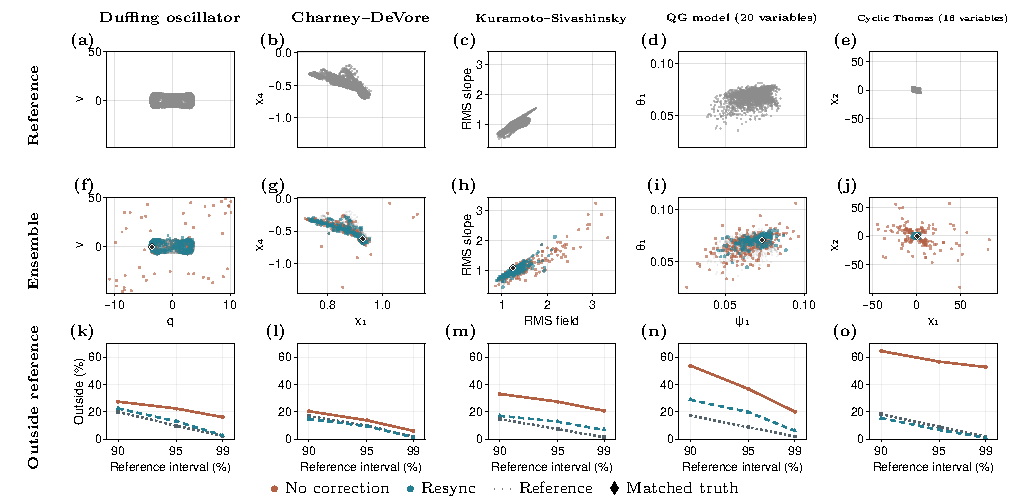
\includegraphics[width=\linewidth,height=.68\textheight,keepaspectratio]{figures/fig02.pdf}
\caption{\textbf{Population structure and reference-envelope exceedance.} Columns identify systems. Panels (a--e) show calibration states and (f--j) all 300 returned members at the midpoint of base interval 40. Marker area encodes projected multiplicity; diamonds mark matched truth. Panels (k--o) give the fraction outside rectangular reference envelopes at the same instant, using 90\%, 95\% and 99\% marginal intervals of the displayed coordinates. Gray curves show calibration-check exceedance. Exceedance panels share a 0--70\% vertical axis; state-coordinate ranges differ by system. Duffing state axes are signed-log; other axes are linear. Envelope definitions and sampling appear in Sect.~\ref{app:note3}.}\label{fig:main-population-views}
\end{figure}

\begin{figure}[!htbp]
\centering
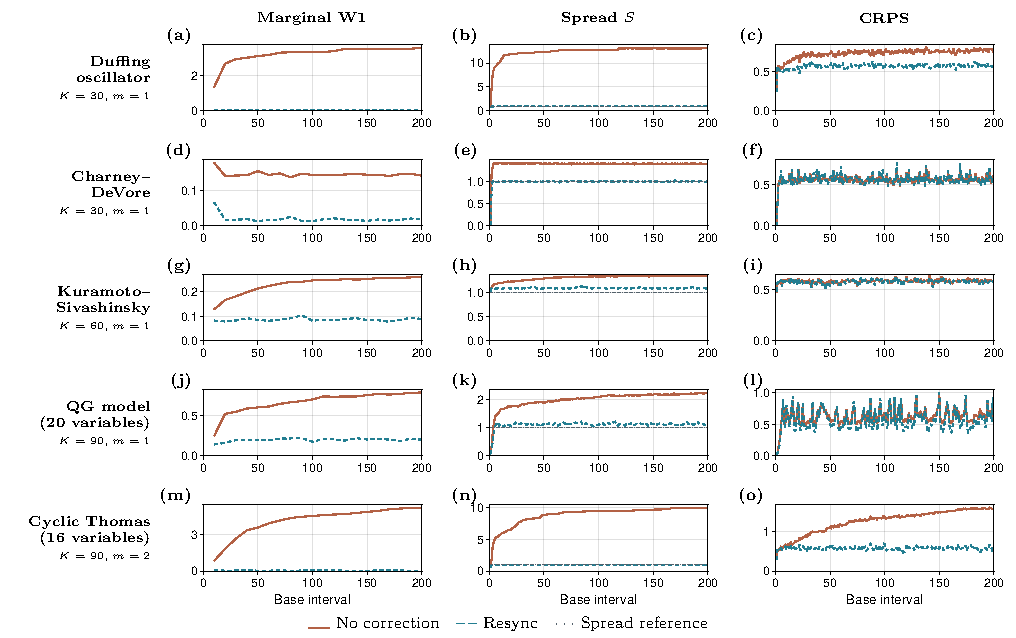
\includegraphics[width=\linewidth,height=.68\textheight,keepaspectratio]{figures/fig03.pdf}
\caption{\textbf{Returned-ensemble quality over the full test.} Panels (a--c), (d--f), (g--i), (j--l) and (m--o) show Duffing, CDV, KS, QG and Thomas, respectively; columns show marginal W1, spread and CRPS for 300 members over $200\tau_0$. Solid curves denote no correction and dashed curves Resync with validation-selected parameters, using the same initial cohort and test trajectory. W1 uses nonoverlapping ten-base-interval windows; spread and CRPS use one-base windows. Dotted lines mark calibration spread references. All axes are linear and start at zero. Each case uses one model bank and one physical test trajectory; successive windows are not independent repetitions.}
\label{fig:main-case-curves}
\end{figure}


\subsection{Illustrative autonomous continuations}
Figure~\ref{fig:resync-sequential-examples} illustrates resync in Duffing-trained LSTM and reservoir models. The same recipient is shown during its initial autonomous rollout and in matched continuations with no intervention or resync. In the LSTM example, a trajectory confined to one well under continued autonomous prediction returns to trajectories visiting both wells after resync. The reservoir example likewise moves closer to the reference state distribution. These selected validation continuations illustrate finite-window changes in own behavior; they are not estimates of sustained member recovery or architecture performance. All displayed continuations are generated by the recipient's own fixed model, without current-record replacement. Sect.~\ref{app:note12} gives model settings, selection criteria and evaluation scope.
\begin{figure}[!htbp]
\centering
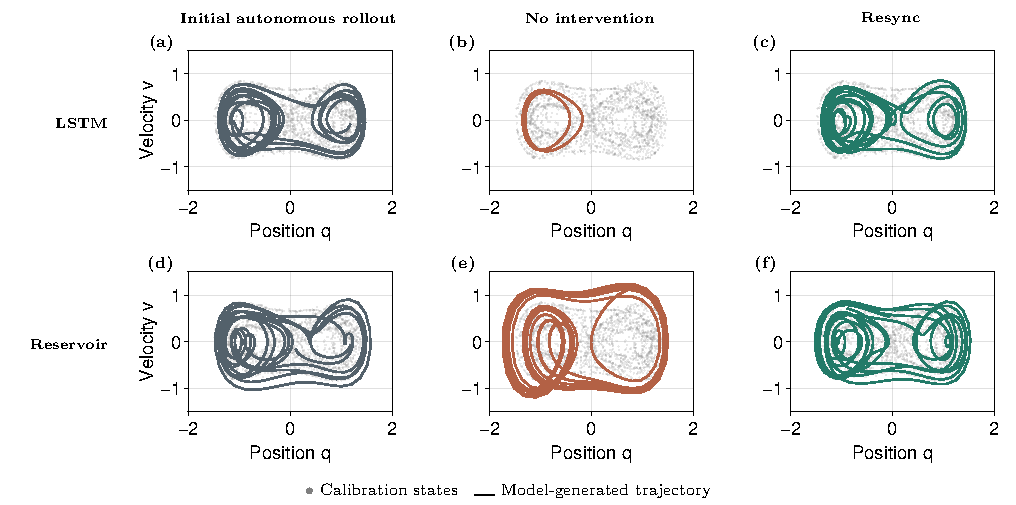
\includegraphics[width=\linewidth,height=.68\textheight,keepaspectratio]{figures/fig04.pdf}
\caption{\textbf{Resync in Duffing-trained sequential models.} Rows show an LSTM (a--c) and a reservoir model (d--f); columns show initial autonomous rollout, no intervention and Resync. Each panel spans 1,000 steps and shows the recipient's own model output, with fixed parameters and no current-record replacement. Gray points are calibration states. All six panels use identical physical-coordinate limits and panel sizes. These selected validation examples illustrate application; Sect.~\ref{app:note12} records the model settings and example-selection rule.}
\label{fig:resync-sequential-examples}
\end{figure}


\subsection{Matched interventions in Duffing and KS}
At each of 199 boundaries of the full-policy trajectory, we fork the same ensemble history and recipient--donor schedule into four state/input conditions. Outcomes score the next own segment at ensemble level before record replacement, rather than classify individual-recipient recovery. These are dependent events within one bank and trajectory per system, not independent replicates.
\begin{table}[!htbp]\caption{Matched next-own-segment means. The factors are donor boundary input ($b$) and donor-history reconstruction ($r$). W1 uses one intervention segment, unlike the ten-base windows of Table~\ref{tab:main-case-results}. The $b=0,r=1$ condition deliberately uses the old own boundary input with a reconstructed state.}\label{tab:matched-controls}
\centering\small\begin{tabular}{lccrr}\toprule System & $b$ & $r$ & W1 & CRPS\\\midrule
Duffing & 0 & 0 & 0.801 & 0.581\\
Duffing & 1 & 0 & 2.016 & 0.631\\
Duffing & 0 & 1 & 2.043 & 0.633\\
Duffing & 1 & 1 & 0.288 & 0.571\\
KS & 0 & 0 & 0.113 & 0.577\\
KS & 1 & 0 & 0.101 & 0.577\\
KS & 0 & 1 & 0.113 & 0.577\\
KS & 1 & 1 & 0.100 & 0.576\\
\bottomrule\end{tabular}\end{table}
In Duffing, the aligned full intervention improves both scores relative to either isolated factor. In KS, the full intervention and boundary-input-only condition are much closer. The factorial contrast is descriptive and depends on the chosen score and the deliberately mismatched continuation in one branch; it does not establish a universal interaction mechanism. Event-wise contrasts and their empirical quartiles are given in Sect.~\ref{app:note5}.


\subsection{Climatology and maintenance diagnostics}
Against a static empirical climatology built from the disjoint calibration target, selected-policy CRPS differs by approximately $-0.95\%$ to $+0.95\%$. These small full-period differences are descriptive and do not show uniform superiority to climatology. Sect.~\ref{app:note10} gives system-specific values and a reference accounting for finite ensemble size.

All returned test outputs are finite and scoring truth is complete. Auxiliary checks reveal remaining limitations: for example, QG's coordinate-wise coverage deviation increases despite mean coverage approaching nominal. Constant-output counts, coverage and correlation-based effective dimension are reported in Sect.~\ref{app:note10}.

Additional Duffing and KS ensemble realizations and physical starts reproduce the direction of the paired ensemble-score improvements in a targeted consistency check (Sect.~\ref{app:note13} and Fig.~\ref{fig:crossed-replication}). Replay-length quality--cost curves are provided in Supplementary Fig.~\ref{fig:duffing-replay-cost}.

\section{Discussion}

\subsection{Resync and ensemble maintenance.}
Resync reduces marginal-distribution and spread losses in the five tested reservoir settings. CRPS changes less and is not uniformly improved over climatology. Comparing autonomous candidates with returned records is consequential: resync changes subsequent model behavior as well as the population of issued outputs. A visible return toward the reference states therefore needs to be assessed alongside distributional and probabilistic scores.

Identifying erroneous members does not guarantee an ensemble gain: removing an outlier can leave a biased population. Exact counterexamples in Sect.~\ref{app:note9} distinguish member screening from population-level improvement.

\subsection{Applicability to sequential models.}
The Duffing LSTM example illustrates that the resync operation can be applied beyond reservoirs (Fig.~\ref{fig:resync-sequential-examples}). Input-driven state reconstruction is compatible with other recurrent architectures \citep{lu2018attractor,vlachas2018lstm}; the example does not establish their comparative performance or general recovery rate. The required amount of history and the role of the boundary input may depend on the model. Increasing the intervention fraction does not necessarily improve ensemble quality: in the illustrative LSTM validation runs, larger fractions worsen returned W1 and CRPS (Sect.~\ref{app:note12}).

\subsection{Generated paths and climatology.}
Static climatology provides a one-time marginal benchmark for CRPS. We do not infer path-based forecasting skill from marginal improvements: that would require temporal validation and path-based comparators. Sect.~\ref{app:note11} discusses the distinction and the information advantage of ideal conditional forecasts.

\subsection{State intervention without parameter adaptation.}
Sharing histories in observation space permits recipients with different internal coordinates to process the same donor history without retraining or additional observations. This redistributes information already represented by the learned ensemble; it does not remove shared biases or guarantee correct autonomous dynamics. Full-history resync is defined without assuming fading memory. Echo-state conditions may motivate shorter histories \citep{jaeger2001echo,yildiz2012revisiting,platt2021robust}, but do not guarantee improved ensemble quality.

\subsection{Mechanism of resync.}
The implemented resync combines history replay, which reconstructs the recipient state, with the donor's boundary output as the first input when autonomous prediction resumes. These operations can be separated to examine their respective roles. The matched next-own-segment controls show a strong score interaction in Duffing and a much smaller difference between the full and boundary-only interventions in KS (Table~\ref{tab:matched-controls}). These score-dependent contrasts do not establish a universal interaction law; the history-only diagnostic also introduces an inconsistent boundary input. Sect.~\ref{app:note5} gives event-wise summaries and the complete protocol.

\subsection{Cost and scope.}
Avoiding retraining does not imply inexpensive inference: full-history replay adds substantial rollout overhead (Sect.~\ref{app:note10}). The replay-length analysis in Sect.~\ref{app:note13} and Fig.~\ref{fig:duffing-replay-cost} identifies a quality--cost trade-off: shorter histories retain similar scores in Duffing and match the stored full-history diagnostics over a range of tested lengths in KS. Replay length was not selected using these test outcomes. Joint validation of replay length, correction fraction and interval, together with adaptive replay termination, is left for future policy research.

Gains are measured against the baseline at the chosen reservoir capacity. The KS example illustrates maintenance of a capacity-limited ensemble, not superiority to a larger uncorrected reservoir; the separate capacity pilot and larger-reservoir outcomes are retained in the reproducibility record. Two validation starts are temporal blocks, and each primary test uses one reservoir bank and one separately seeded physical trajectory. No independent-bank uncertainty interval or universal improvement claim follows from these comparisons. Marginal agreement, nominal average coverage and low CRPS alone do not establish joint-distribution fidelity, conditional calibration or correct temporal dynamics.




\conclusions
Generated-history intervention connects the state of a fixed recipient model to its subsequent autonomous outputs and the quality of a returned ensemble. The tested reservoir policies improve marginal-distribution and spread losses, while probabilistic scores and auxiliary diagnostics show that these changes do not imply uniform ensemble improvement. Matched continuations distinguish changes in model-generated behavior from replacement of the current output record, with different additional history effects in Duffing and Kuramoto--Sivashinsky. Supporting analyses assess ensemble-level consistency and replay cost. Joint replay-length selection and adaptive intervention remain future policy questions, and sustained recovery requires separate assessment.

\appendix
\section{Supporting methods and analyses}
\subsection{Additional diagnostics}\label{app:note1}
The test records include 50\% and 90\% coverage, coordinate-wise coverage deviations, correlation-based effective dimension and constant/nonfinite exclusion counts.
\subsubsection{Correlation-based effective dimension.}
Sample $q\le\min\{64,T_b\}$ unique evenly spaced times, including endpoints, from a base window of $T_b$ samples. Stack each member's coordinate-wise time-demeaned standardized outputs into $\mathbf z_i$. For $n$ eligible members,
\begin{equation}
C_{ij}=\frac{\langle\mathbf z_i,\mathbf z_j\rangle}{\|\mathbf z_i\|\|\mathbf z_j\|},\qquad
N_{\rm eff}=\frac{(\sum_k\lambda_k)^2}{\sum_k\lambda_k^2}
=\frac{n^2}{\|C\|_F^2},
\end{equation}
where $\lambda_k$ are the eigenvalues of $C$ \citep{pennell2010number}. Values lie between one and $\operatorname{rank}(C)\le\min\{n,D(q-1)\}$. The measure captures linear similarity: scaling, coordinate offsets and anticorrelation can reduce effective dimension without counting exact copies or testing independence.

A member is numerically constant when the RMS of its demeaned samples is below $10^{-10}$. If any correlation is undefined, the full-population score is undefined; a separately labelled subset score reports its member count and constant/nonfinite exclusions. References use the same sampling and eligible count. This numerical convention is not a physical-failure criterion.

\subsubsection{Coverage.}
For coordinate $d$ and window $b$, let $c_{d,b}$ be the fraction of matched truth values inside the central 90\% empirical interval. Report $D^{-1}\sum_d c_{d,b}$ and $D^{-1}\sum_d|c_{d,b}-0.9|$; analogous summaries use nominal 50\%. Forty-interval results average base-window values. Empirical quantiles use Hyndman--Fan type 7 ($\alpha=\beta=1$). Coordinate-wise absolute deviations avoid cancellation but retain finite-sample variability. These are marginal checks with autocorrelated times, not initial-state-conditional calibration tests \citep{gneiting2007calibration}.


\subsection{Reference construction}\label{app:note2}
Calibration is disjoint from training, validation and test. Training-derived coordinate transforms are used throughout. Within calibration, the W1 target bank, population-window pool and coverage check targets have separate roles (Sect.~\ref{app:note7}).

Reference ensembles match the evaluated window length, member count, sampling and normalization. For each draw, sample $N$ nonoverlapping windows without replacement from the population pool, randomize the grid phase and align relative times. Use 512 draws for base-window indicators and 128 for $10\tau_0$ distribution windows, with seed 20261125. Windows may recur across draws. Report medians and empirical 5--95\% ranges. These are conditional reference ranges, not confidence intervals across independent runs; nonoverlapping windows need not be independent. If fewer than $N$ matching windows are available, the reference is unavailable.

Spread fitting draws define median $S_{\rm ref}$; separate check draws estimate $|\log(S/S_{\rm ref})|$ variability. W1 draws are compared with the target bank, and reference coverage uses held-out truth windows. Mean matching reference losses, bounded below by $10^{-12}$, supply the calibration components of selection scales. They are descriptive loss scales rather than universal error floors. Reference summaries and data lengths appear in Sect.~\ref{app:note7}; complete draw summaries accompany the data.

Effective-dimension references use the same base-window duration and sampled times as model outputs; eligible subsets require the same member count. Forty-interval summaries average window values rather than recomputing pooled scores. Reference agreement establishes neither joint-distribution fidelity nor physical initial-condition uncertainty.

\subsection{Records, sampling and validity}\label{app:note3}
\subsubsection{Initialization and paired cohorts.}
Policies share trained models and forecast-initialized states. Blind initial refill scores first-base candidates and fixes the cutoff at the 30th-largest score among the initial 300 members. Candidates at or above this cutoff are replaced from 150 reserve models, with scores recomputed until the retained pool passes; exhausting the reserve without convergence stops preparation. The 10\% setting defines the cutoff, not the eventual replacement fraction, and is separate from operational correction. All paired policies use the same resulting cohort. Model IDs, checkpoint hashes and initialization indices are recorded; the first 300 models cannot substitute for a refilled cohort.

For fresh origin $o$, initialization uses $\min(1000,o-1)$ preceding observed samples and leaves the boundary observation as the first forecast input. The first validation origin therefore uses 999 warm-up samples; test uses 1000. Stored training endpoints are excluded from this initialization. Missing and unfinished scoring windows are counted without interpolation. 

\subsubsection{Record conventions.}

Own records retain preselection candidates; returned records include donor replacement. Probability scores use the full returned population, while own-output failures remain separately recorded. Order nonselected donors $g_1,\ldots,g_q$ by member index and assign recipient $j$ to $g_{1+(j\bmod q)}$.

Spread uses native-resolution member variance within $\tau_0$ windows; W1 uses full $10\tau_0$ windows. Probability scores use stride $\max(1,\lfloor\tau_0/20\rfloor)$. Forty-interval summaries average forty base-window or four distribution-window values. Sampled diagnostics use identically sampled references.

Any nonfinite returned output invalidates a configuration for selection. Negative, nonfinite or undefined selection losses are invalid; zero loss is allowed, but spread and its reference must be positive. Undefined auxiliary correlations do not invalidate otherwise defined primary scores. A nonfinite baseline prevents baseline-normalized selection. Constant-output flags and finite reference-envelope excursions are not automatic physical failures. Matching initial own-prediction hashes verify paired initialization, not equality of later trajectories.

\subsubsection{Visualization.}
For the KS state-space view, each instantaneous field is represented by $a=(D^{-1}\sum_j u_j^2)^{1/2}$ and $g=(D^{-1}\sum_j [(u_{j+1}-u_{j-1})/(2\Delta x)]^2)^{1/2}$, with periodic indices and $\Delta x=L/D$. These describe field amplitude and roughness and are unchanged by cyclic grid shifts. They are visualization coordinates, not new optimized losses or estimates of dynamical invariants. All 300 returned members enter the state and exceedance views with equal weight, retaining duplicate members. All five systems use the midpoint of base interval 40. Reference point clouds contain 5000 fixed calibration samples. Replayed prefix metrics and first-own hashes match the corresponding completed main tests; the visualization does not change numerical scoring grids.

\subsubsection{Reference-envelope exceedance in the displayed projection.}
This descriptive diagnostic was added after the primary tests and is not used for parameter selection. Split the 5000 calibration visualization points deterministically into two disjoint interleaved sets of 2500 points. The first defines marginal quantiles $Q_j$ and the second supplies the empirical reference-check fraction. Temporal independence of these points is not assumed. For the two displayed coordinates and marginal central-interval level $c\in\{0.90,0.95,0.99\}$, define
\begin{equation}
\mathcal B_c=\prod_{j=1}^2\left[Q_j\!\left(\frac{1-c}{2}\right),Q_j\!\left(\frac{1+c}{2}\right)\right],\qquad
f_{\rm out}(c)=\frac1N\sum_{i=1}^N\mathbf1\{x_i(t_*)\notin\mathcal B_c\}.
\end{equation}
Quantiles use linear interpolation between ordered samples. The reference curve uses the check set in place of model members. Here $c$ specifies each marginal interval, not the joint coverage of the rectangular region; a 99\% interval in each coordinate need not give 1\% joint exceedance. Nonzero reference exceedance is expected. Curves use the same levels for all systems and independently scaled linear percentage axes. Leaving the envelope does not certify an erroneous trajectory, and reducing tail mass below the reference is not automatically an improvement. Rare valid states and joint or temporal errors inside the envelope are not resolved by this diagnostic. These snapshot fractions do not establish forecast calibration or sustained recovery.

\subsection{Parameter selection}\label{app:note4}
Each system evaluates twelve corrected settings from the 21-point grid at two validation origins, plus a shared no-correction forecast at each origin. The initial design is $(K,m)=(30,1),(6,2),(60,4),(90,1)$.

A GP fits finite valid losses, including the baseline. At each proposal, a weight is drawn from $\{0.1,0.3,0.5,0.7,0.9\}$ using the execution seed plus history length (seed 20261122 for Duffing/CDV; 20261123 for KS/QG/Thomas). Normalized losses are combined by augmented Chebyshev scalarization with the observed componentwise ideal and augmentation 0.05, then log-transformed and standardized. A Mat\'ern-5/2 kernel selects length scale from $\{0.2,0.5,1,2\}$ and diagonal noise from $\{10^{-6},10^{-3},0.03\}$ by marginal likelihood. Final parameter selection uses the minimax rule in Methods.

Failures remain validity records rather than numerical penalties. Acquisition weights expected improvement by
\begin{equation}
\pi(c)=\frac{1+\sum_i w_i(c)\mathbf1\{i\text{ valid}\}}{2+\sum_i w_i(c)},
\end{equation}
where $w_i$ is a Mat\'ern-5/2 kernel of length scale 0.5 on the log-count/log-interval coordinates. This smoothed success weight uses all observed settings. Every fourth acquisition after the initial design instead maximizes posterior standard deviation times $\pi(c)$. With fewer than two valid observations, acquisition uses distance to the nearest observed setting times $\pi(c)$. Previously evaluated settings are not repeated. An invalid paired baseline prevents selection; process errors stop execution.


\subsubsection{Final selection and numerical rules.}
For loss $j$, use $a_j=\max\{L_j(0),\delta_j\}$, with $0$ denoting no correction and $\delta_j$ the larger of the mean matching calibration check loss and $10^{-12}$. Calculate scales after baseline evaluation and before corrected candidates; all candidates share them. The selected valid setting minimizes $\max_j L_j(c)/a_j$. Ties satisfy $|Q-Q_{\min}|\le10^{-10}+10^{-6}|Q_{\min}|$ and prefer no correction, then smaller $K/m$, smaller $K$ and smaller $m$. The baseline score need not equal one when a calibration scale exceeds its loss. Calibration scales describe finite-window reference variability, not universal error floors. Auxiliary outcomes are not directly optimized and need not be statistically independent of W1 or spread.

Validity gates follow Sect.~\ref{app:note3}; finite-member substitution and numerical failure penalties are not used.

Validation selects the correction fraction and interval, which are then held constant during the $200\tau_0$ test. Figure~\ref{fig:validation-selection} shows the evaluated settings; losses, validity and scales are retained in the accompanying records.

\begin{figure}[!htbp]
\centering
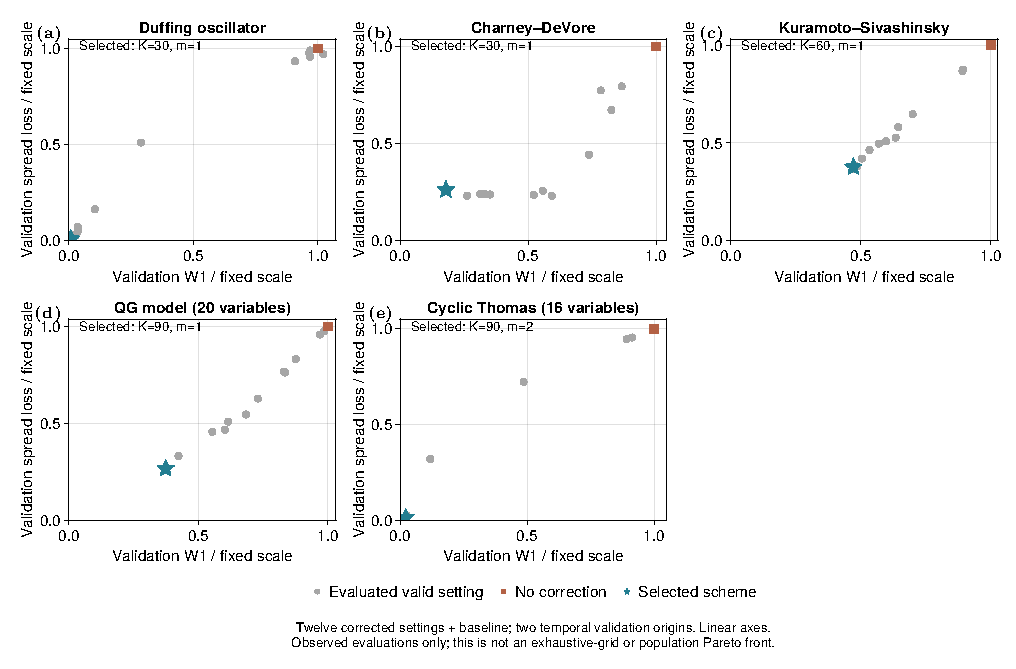
\includegraphics[width=\linewidth,height=.68\textheight,keepaspectratio]{figures/figA01.pdf}
\caption{Validation evaluations for the five systems, with W1 and spread losses divided by their baseline/calibration-derived scales. Axes are linear. Gray circles denote valid evaluations, squares no correction and stars the minimax selections. Each search evaluates twelve corrected settings at two temporal origins; this is not an exhaustive grid or population Pareto front. CRPS is not used for selection.}\label{fig:validation-selection}
\end{figure}

\subsection{Boundary-input and history-replay controls}\label{app:note5}
The factors are donor boundary-input transfer $b$ and history-state reconstruction $r$. Current-record replacement is held common; the primary outcome is the next own segment before further replacement.

\begin{center}\small
\begin{tabularx}{\textwidth}{ccXX}
\toprule
$b$ & $r$ & Boundary state & First input \\ \midrule
0 & 0 & Own endpoint & Own endpoint output \\
1 & 0 & Own endpoint & Donor endpoint output \\
0 & 1 & Donor-history reconstruction & Old own output (mismatched) \\
1 & 1 & Donor-history reconstruction & Donor endpoint output \\
\bottomrule\end{tabularx}
\end{center}

For a common-window score $Y_{br}$, conditional contrasts and interaction are
\begin{align}
\Delta_{R\mid B=1}&=Y_{11}-Y_{10}, & \Delta_{B\mid R=0}&=Y_{10}-Y_{00},\\
\Delta_{B\mid R=1}&=Y_{11}-Y_{01}, & \Delta_{BR}&=Y_{11}-Y_{10}-Y_{01}+Y_{00}.
\end{align}
Compute nonlinear scores before taking contrasts. The $(0,1)$ branch intentionally combines a replayed state with an inconsistent old input; it is not a natural replay-only continuation. No branch changes model weights.

Controls use the original Duffing ($K=30,m=1$) and KS ($K=60,m=1$) test trajectories, 300-member cohorts and selected parameters, without repeating BO or training. Repeated policies span $200\tau_0$ and allow recipient/donor schedules to evolve. Conditional forks instead share the parent history, recipients and donors at each boundary except the last, and evaluate the next own segment. Fork W1 uses one intervention segment, distinct from the primary ten-base window. The aligned fork is checked against the next parent candidate; baseline and full-policy outputs are checked against the original tests. Preliminary ten-base checks precede full execution.

Any nonfinite own output invalidates a control branch, unlike the returned-output gate of the primary evaluation. Exploratory records include lead-wise CRPS and within-segment correlations at lags $1$, $\max(1,\lfloor\tau_0/10\rfloor)$ and $\max(1,\lfloor\tau_0/2\rfloor)$, with constant/nonfinite exclusion counts. Segments are not concatenated. These diagnostics do not establish cross-boundary continuity and are not used for retuning. The completed paired-event results are reported below; they quantify conditional score contrasts rather than independent-run generalization.
\subsubsection{Completed matched-event results.}
Duffing and KS each contain 199 matched events (796 branches), all finite; original full-policy and no-intervention own-score anchors agree to below $10^{-9}$. The original test data and choices are unchanged. For every contrast below, compute the score on each branch first, then subtract within event. The median and interquartile range describe dependent events, not uncertainty across independent runs.
\begin{center}\small\begin{tabular}{llrr}\toprule System/score & Contrast & Mean & Median [Q1,Q3]\\\midrule
Duffing/W1 & $Y_{11}-Y_{10}$ & -1.7279 & -1.7316 [-1.8302,-1.6234]\\
Duffing/CRPS & $Y_{11}-Y_{10}$ & -0.0605 & -0.0601 [-0.0675,-0.0542]\\
KS/W1 & $Y_{11}-Y_{10}$ & -0.0008 & -0.0009 [-0.0041,0.0026]\\
KS/CRPS & $Y_{11}-Y_{10}$ & -0.0003 & -0.0001 [-0.0027,0.0022]\\
\bottomrule\end{tabular}\end{center}
Complete condition summaries, event-wise differences and interaction contrasts are retained in the reproducibility files. No event-level significance test or independent-run confidence interval is inferred. Repeated complete policies have endogenous selection schedules and are distinct from these common-parent forks.

\begin{figure}[!htbp]
\centering
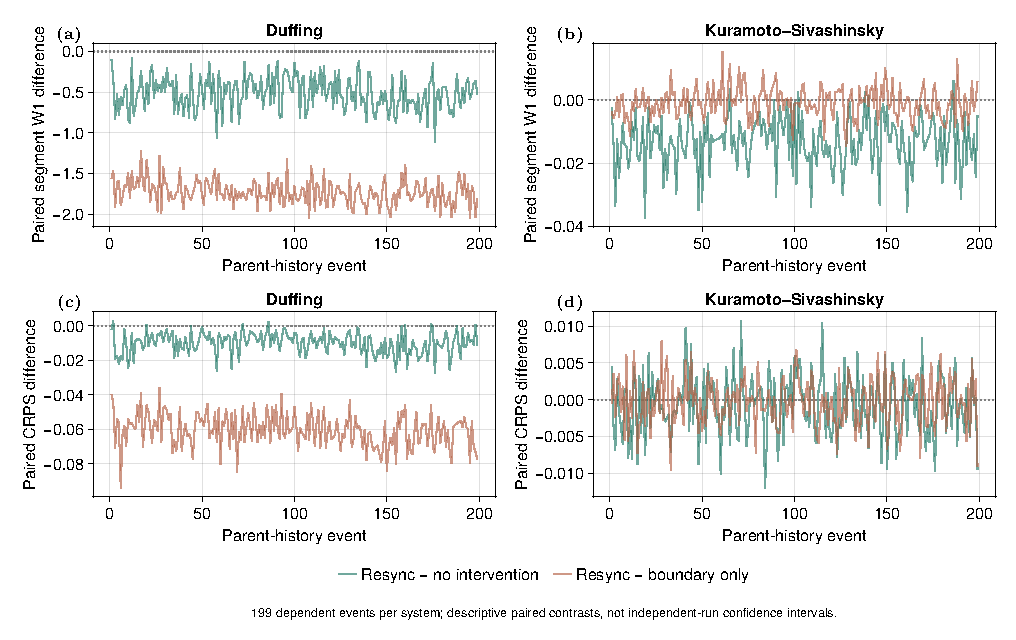
\includegraphics[width=.95\linewidth,height=.68\textheight,keepaspectratio]{figures/figA02.pdf}
\caption{Event-wise score differences on a common parent history. Each curve follows the 199 successive update events of one model bank and physical trajectory. Green compares full Resync with no state/input intervention; copper compares full Resync with boundary input alone. Scores use the next own segment. Axes are linear, and panels use their own score ranges. Event variation is descriptive and is not an independent-run confidence interval.}\label{fig:paired-event-contrasts}
\end{figure}


\subsection{Evaluation scope}\label{app:note6}
System presets and earlier validation outcomes were inspected during development. The present losses were specified before the new validation runs and separately seeded tests. Earlier snapshot-based losses, fair-CRPS diagnostics and other-model feasibility tests remain versioned in the archive; they are not combined with current test scores.

% Current settings read from frozen manifests; earlier evidence below retains its original scope.
\subsection{Data, model settings and empirical references}\label{app:note7}
Calibration comprises a $400\tau_0$ target bank, a $20\tau_0$ gap, a $3200\tau_0$ population pool, another $20\tau_0$ gap and $400\tau_0$ of checks. Validation initialization and targets use fresh continuation data; the original training prefix is retained unchanged.

\begin{table}[htbp]\caption{Data lengths in saved samples. Calibration and fresh validation exclude the stored training prefix; test lengths cover scored forecasts.}\label{tab:v4-data}
\centering\small\begin{tabular}{lrrrrr}\toprule
Case & Train & Base & Calibration & Fresh validation & Test\\\midrule
Duffing & 5000 & 600 & 2424000 & 62000 & 120000 \\
CDV & 20000 & 223 & 900920 & 24300 & 44600 \\
KS & 20000 & 474 & 1914960 & 49400 & 94800 \\
QG & 20000 & 217 & 876680 & 23700 & 43400 \\
Thomas & 10000 & 100 & 404000 & 12000 & 20000 \\
\bottomrule\end{tabular}\end{table}
The calibration, validation and test seeds are 2026112211, 2026112212 and 2026112213 for Duffing/CDV, 2026112211, 2026112322 and 2026112223 for KS, 2026112341, 2026112342 and 2026112343 for QG and 2026112351, 2026112352 and 2026112353 for Thomas. Distinct seeds establish nonreuse, not independent physical replicates. Initialization follows Methods.

\begin{table}[htbp]\caption{Reservoir presets. All use sparse reservoirs, degree 6, washout 500 and seed start 1234. Each 300-member cohort is selected from 450 models. Training-input noise has standard deviation $10^{-6}$; evaluation truth is noise-free.}\label{tab:v4-training}
\centering\small\begin{tabular}{lrrrrr}\toprule
Parameter & Duffing & CDV & KS & QG & Thomas\\\midrule
Reservoir units & 200 & 500 & 200 & 500& 400\\
Leak & 0.3 & 0.3 & 0.9 & 0.5& 1.0\\
Spectral radius & 0.9 & 0.9 & 0.4 & 0.5& 0.1\\
Input scale & 0.1 & 0.1 & 0.1 & 0.1& 2.0\\
Bias scale & 0.0 & 0.5 & 0.9 & 0.5& 2.0\\
Ridge & 1e-06 & 1e-06 & 0.001 & 1e-06& 1e-06\\
Readout map & linear & nlat1 & nlat2 & nlat1& linear\\
Model normalization & no & yes & yes & yes& yes\\
\bottomrule\end{tabular}\end{table}
Readout-map identifiers refer to the transformations in the implementation; only readout weights are fitted. Thomas assigns one input coordinate per reservoir unit, with balanced shuffled coordinate counts and weights uniform on $[-2,2]$. Evaluation always uses training-only population standard deviations, distinct from model-input normalization. Paired policies share trained models and initial members.

The Duffing preset has $(\alpha,\beta,\delta,\gamma,\omega)=(1,1,0.3,0.4,1.2)$ with saved/integration steps $0.1/0.001$. CDV uses parameters $(C,b,\beta,\gamma,x_1^*,x_4^*)$ with values $(0.1,0.5,1.25,0.2,0.95,-0.76095)$ and steps $1/0.05$. KS uses $L=22$, $\nu=1$, 64 observed grid values and steps $0.25/0.05$. QG uses a wavenumber-two truncation in both horizontal coordinates, retaining ten barotropic and ten baroclinic coefficients in \texttt{qgs} v1.0.0 \citep{demaeyer2020qgs}, saved/RK4 integration steps $0.5/0.1$, and transient duration 200000. No POD is applied; the parameter dump and tendency tensor accompany the data. Thomas uses $\dot x_j=\sin(x_{j+1})-0.18x_j$ with cyclic indexing over 16 coordinates, saved/RK4 integration steps $0.2/0.02$, and transient duration 500. 

\begin{table}[htbp]\caption{Spread references and calibration loss scales (Sect.~\ref{app:note2}). The loss scales are descriptive, not universal error floors.}\label{tab:v4-calibration}
\centering\small\begin{tabular}{lrrr}\toprule
Case & $S_{\rm ref}$ & $\delta_W$ & $\delta_S$\\\midrule
Duffing & 0.990859 & 0.002402 & 0.001179 \\
CDV & 0.998778 & 0.004246 & 0.003954 \\
KS & 1.001032 & 0.045266 & 0.001297 \\
QG & 1.003106 & 0.023285 & 0.013573 \\
Thomas & 1.001921 & 0.043260 & 0.003108 \\
\bottomrule\end{tabular}\end{table}

\subsection{Earlier own/returned trade-offs}\label{app:note8}
Two exploratory Duffing comparisons used 20 members over eight intervals (A, temporal origin 1) and 60 members over twenty intervals (B, origin 2). Their original and modified policies are complete interventions, not isolated replay controls. Own W1 improves under the modified policies, whereas returned W1 changes little in A and worsens in B; returned spread loss increases in both. All additional pilot arms remain in the versioned records.

\begin{table}[htbp]
\caption{Contrasting arms of the earlier Duffing pilots. Spread loss uses the archived intervalwise absolute log ratio with reference 1.0002542500642428, distinct from the current base-window loss.}
\label{tab:legacy-population}
\centering\small\begin{tabular}{llrrr}\toprule
Pilot & Policy & Own W1 & Returned W1 & Spread loss \\ \midrule
A & Original & 0.58964 & 0.08891 & 0.08179 \\
A & Repair-fixed & 0.15743 & 0.08427 & 0.09274 \\
B & Original & 0.20184 & 0.07148 & 0.04515 \\
B & Population-fixed & 0.09597 & 0.07802 & 0.05643 \\
\bottomrule\end{tabular}\end{table}
These previously inspected results illustrate a lack of joint improvement, not its mechanism or frequency. They are not current held-out tests.

\subsection{Oracle removal does not guarantee ensemble improvement}\label{app:note9}
At truth $y=0$, removing $+2$ from $[-1,-1,2]$ lowers member-average absolute error from $4/3$ to $1$ but raises empirical CRPS from $2/3$ to $1$; the retained predictions are one-sided.

For a distributional example, let truth follow $U[-1,1]$. Of 300 forecasts, 100 equal $+2$; the remaining 200 are balanced uniform quantiles, identical $-1$ values, or distinct quantiles in $[-1,-0.8]$. An oracle removes exactly the out-of-support values, with no false positives. Expected scores and coverage are calculated analytically.

\begin{table}[htbp]
\caption{Oracle removal under uniform truth. W1 and expected empirical CRPS are lower-is-better; coverage is compared with nominal 90\%. Expectations integrate over $U[-1,1]$.}
\label{tab:oracle-removal}
\centering\scriptsize
\begin{tabular}{llrrrr}
\toprule
Remaining population & Arm & N & W1 & Expected CRPS & Coverage90 \\ \midrule
Balanced & Before & 300 & 0.666668 & 0.518519 & 92.27\% \\
Balanced & After removal & 200 & 0.002500 & 0.333338 & 89.55\% \\
Identical left bias & Before & 300 & 0.888889 & 0.666667 & 100.00\% \\
Identical left bias & After removal & 200 & 1.000000 & 1.000000 & 0.00\% \\
Distinct left bias & Before & 300 & 0.822222 & 0.611852 & 99.23\% \\
Distinct left bias & After removal & 200 & 0.900000 & 0.873334 & 8.96\% \\
\bottomrule\end{tabular}
\end{table}



Removing impossible forecasts improves the balanced case but worsens both biased cases. The oracle certifies the removed values, not the representativeness of the retained ensemble. CRPS uses the finite empirical $N^2$ denominator. These examples disprove a universal improvement guarantee; removal, record replacement and replay remain distinct interventions.

\subsection{Auxiliary outcomes and additional tests}\label{app:note10}
All primary tests contain 200 base windows and twenty distribution windows per policy, with finite returned outputs and no missing scoring truth. Paired initial own-prediction hashes agree. Each case uses one model bank and one physical test trajectory.

\begin{table}[htbp]\caption{Auxiliary test diagnostics. MAD is mean base-window coordinate-wise absolute deviation from 90\% coverage, in percentage points. Dashes denote undefined full-population effective dimension; exclusion counts remain in the window records.}\label{tab:followup-auxiliary}
\centering\small\begin{tabular}{llrrr}\toprule
System & Policy & Coverage90 & MAD (pp) & $N_{\rm eff}$\\\midrule
Duffing & No correction & 99.74\% & 9.79 & --- \\
Duffing & Resync & 89.50\% & 4.00 & 12.79 \\
CDV & No correction & 90.99\% & 5.06 & --- \\
CDV & Resync & 88.94\% & 5.76 & 17.62 \\
KS & No correction & 97.95\% & 8.13 & --- \\
KS & Resync & 93.51\% & 5.65 & 55.31 \\
QG & No correction & 96.36\% & 10.18 & --- \\
QG & Resync & 89.53\% & 12.55 & 17.57 \\
Thomas & No correction & 99.92\% & 9.98 & --- \\
Thomas & Resync & 88.84\% & 11.76 & 17.73 \\
\bottomrule\end{tabular}\end{table}
Mean coverage approaches nominal in QG and Thomas while coordinate-wise MAD increases. Average coverage therefore does not establish coordinate calibration. At least one numerical constant-member flag occurs in 193, 197, 198, 192 and 197 baseline windows for Duffing, CDV, KS, QG and Thomas, respectively. Resync returned records have none; own records retain seven flagged KS windows and seventeen Thomas windows. These are counts of windows containing at least one flagged member, not counts or fractions of failed members. Flags are numerical exclusions, not physical-failure labels. Member-wise counts, unique flagged slots and consecutive-flag durations require the separately retained identity-level diagnostics (Sect.~\ref{app:note13}). The reported effective dimensions are correlation-concentration diagnostics; the nominal population of 300 is not an empirical no-correction reference, and the undefined baseline values do not establish a decline from 300.

\subsubsection{Window counts, member counts and matched references.}
The mean constant-member count per window and the maximum below are calculated from the original returned-window exclusion counts. They are not counts of unique affected models. Unique-slot occurrence and consecutive flags are not reconstructible from these aggregate records.
\begin{center}\small\begin{tabular}{lrrrr}\toprule Case & Baseline mean & Baseline max & Resync mean & Ref. $N_{\rm eff}$ median [5--95\%]\\\midrule
Duffing & 64.9/300 & 86/300 & 0/300 & 17.2 [16.8,17.5]\\
CDV & 10.9/300 & 13/300 & 0/300 & 20.1 [18.5,21.6]\\
KS & 38.6/300 & 49/300 & 0/300 & 48.7 [46.5,50.7]\\
QG & 52.4/300 & 79/300 & 0/300 & Unavailable\\
Thomas & 174.2/300 & 227/300 & 0/300 & Unavailable\\
\bottomrule\end{tabular}\end{center}
The available reference uses the same 300-member base-window sampling convention as the model diagnostic. Its interval describes calibration draws, not a confidence interval for model runs. Model scores are means across windows, so comparison with the reference draw distribution is descriptive rather than a formal mean-level test. QG and Thomas calibration summaries do not contain this reference; no substitute value is inferred. Undefined full-population baseline dimensions remain undefined; eligible-subset scores and counts are retained separately.


\subsubsection{Own and returned outputs.}
\begin{table}[htbp]\caption{Own and returned scores over identical test windows. Own candidates include earlier interventions; the contrast does not isolate replay.}\label{tab:own-returned-test}
\centering\small\begin{tabular}{lrrrr}\toprule
Case & Own W1 & Returned W1 & Own CRPS & Returned CRPS\\\midrule
Duffing & 0.28385 & 0.02819 & 0.56919 & 0.56643 \\
CDV & 0.08727 & 0.02028 & 0.56091 & 0.56083 \\
KS & 0.09677 & 0.08686 & 0.57598 & 0.57721 \\
QG & 0.29280 & 0.19835 & 0.57940 & 0.57411 \\
Thomas & 0.12567 & 0.03835 & 0.57477 & 0.57497 \\
\bottomrule\end{tabular}\end{table}

\subsubsection{Static climatology.}
\begin{table}[htbp]\caption{CRPS at matched test times. The iid-300 column is an analytical expectation for independent climatology draws, not a confidence interval or an assumption about reservoir members.}\label{tab:climatology-reference}
\centering\small\begin{tabular}{lrrr}\toprule
Case & Calibration CDF & Expected iid 300 & Selected ensemble\\\midrule
Duffing & 0.57184 & 0.57374 & 0.56643 \\
CDV & 0.56334 & 0.56521 & 0.56083 \\
KS & 0.57343 & 0.57535 & 0.57721 \\
QG & 0.56868 & 0.57048 & 0.57411 \\
Thomas & 0.57370 & 0.57562 & 0.57497 \\
\bottomrule\end{tabular}\end{table}
CRPS for the calibration CDF is evaluated exactly by sorted sums. For $D_F=\frac12\mathbb E_{X,X'\sim F}|X-X'|$, independent sampling with replacement gives expected empirical score $\operatorname{CRPS}(F,y)+D_F/300$. This expectation is not a confidence interval.

Each calibration CDF uses all target-bank samples under the same normalization and scoring times as the ensemble. The reference is not fitted to test truth. These postselection comparisons do not change parameter selection; differences below one percent are descriptive.

\subsubsection{Additional completed cases.}
The larger KS reservoir and MAOOAM56 retain unfavorable changes as well as gains. These outcomes are distinct from the main 200-node KS test.
\begin{table}[htbp]\caption{Additional test changes relative to no correction. Negative values indicate lower loss; KS here uses a 500-node reservoir.}\label{tab:completed-v4-original-set}
\centering\small\begin{tabular}{lrrrr}\toprule
System & $K/m$ & W1 change & Spread-loss change & CRPS change\\\midrule
KS (500 nodes) & $90/2$ & $-9.03\%$ & $-76.65\%$ & $+0.085\%$\\
MAOOAM56 & $3/2$ & $-1.22\%$ & $+4.66\%$ & $-0.563\%$\\
\bottomrule\end{tabular}\end{table}

\subsubsection{Computation.}
For fixed model size, replay over $J$ segments of length $\tau$ requires $O(K\tau J^2)$ state updates. At fixed duration $T=J\tau$, this component scales approximately as $KT^2/\tau$.

Baseline/Resync rollout times are 77.7/755.8\,s for Duffing, 95.6/767.0\,s for CDV, 218.9/8111.4\,s for KS, 110.4/2080.7\,s for QG and 32.5/390.7\,s for Thomas. These exclude scoring and preparation and are not a standardized hardware benchmark.

\subsection{Conditional information, climatology and path tasks}\label{app:note11}
Let $Y_h$ be a future scalar observation, $\mathcal I$ the available forecast information, $G_h(z\mid\mathcal I)$ the true conditional CDF, and $\bar G_h(z)=\mathbb E[G_h(z\mid\mathcal I)]$ its unconditional CDF. Assume finite first moments and expected scores. The CRPS loss is \citep{gneiting2007proper}
\begin{equation}
\operatorname{CRPS}(F,y)=\int_{\mathbb R}\big(F(z)-\mathbf1\{y\le z\}\big)^2\,dz.
\end{equation}
Conditioning at each threshold gives
\begin{equation}
\mathbb E\!\left[\operatorname{CRPS}(\bar G_h,Y_h)\right]
-\mathbb E\!\left[\operatorname{CRPS}(G_h(\cdot\mid\mathcal I),Y_h)\right]
=\int_{\mathbb R}\operatorname{Var}\!\left(G_h(z\mid\mathcal I)\right)dz\ge0.
\end{equation}
For an approximate information-dependent forecast $F_h$, the corresponding excess loss is
\begin{align}
&\mathbb E\!\left[\operatorname{CRPS}(F_h,Y_h)\right]
-\mathbb E\!\left[\operatorname{CRPS}(\bar G_h,Y_h)\right] \nonumber\\
&\qquad=\int_{\mathbb R}\mathbb E\big[(F_h(z)-G_h(z\mid\mathcal I))^2\big]dz
-\int_{\mathbb R}\operatorname{Var}\!\left(G_h(z\mid\mathcal I)\right)dz.
\end{align}
The first term is approximation error; the second is the value of conditional information. Either may dominate, so the identity gives no improvement guarantee for Resync. Independent forecast randomization may be included in $\mathcal I$ when conditionally independent of truth given the original information.

The information term need not decrease monotonically with lead. An exactly known deterministic state and flow yield a point-mass conditional law at every finite lead; a positive Lyapunov exponent alone does not imply convergence to climatology. The reservoir members here are model realizations, not posterior samples of specified physical uncertainty.

A one-time marginal does not specify path statistics. Stationary binary Markov chains can share equal state probabilities while having persistence $a=\Pr(Y_{t+1}=Y_t)$ and mean residence time $1/(1-a)$ for $a<1$. Generated paths therefore require separate temporal validation. Block-resampling climatology is a stronger path comparator than independent marginal draws. Because Resync can introduce boundary changes, within-segment correlations do not establish cross-boundary continuity or correct event durations.

\subsection{Sequential-model illustration}\label{app:note12}
The Duffing illustration uses separate LSTM and ESN validation cohorts, rather than the five primary tests. Inputs are position and velocity, without future forcing phase. The one-layer LSTM has 32 hidden units and a linear next-state readout. Training uses 8,000 samples, 96-step sequences, 16 loss warm-up steps, gradient-norm clipping at 1 and 10,000 Adam updates; the learning rate is $10^{-3}$ through update 3,000 and $3\times10^{-4}$ thereafter. The illustrative ESN has 96 units, spectral radius 0.95, leak 0.5 and ridge coefficient $10^{-4}$. Both use common training-prefix normalization and 1,000 observed initialization samples from a zero state, without initial refill. Parameters remain fixed during prediction and resync.

Each validation uses 300 members, two seed banks and three origins over 40 intervals of 100 steps. Resync uses full generated history; minimum history length is not estimated. Execution seeds, model hashes and data blocks are retained in the reproducibility records. These exploratory outcomes are not new held-out tests.

Main-text Fig.~4 shows selected finite-window autonomous continuations under resync. Recipients meet initial finite-horizon prediction and distribution checks, then depart from calibration-based distribution or autocorrelation ranges. Among events whose matched no-intervention continuation remains outside these ranges while resync returns within them for the final three rolling windows, the first is selected in bank, origin, intervention-time and member-index order. Both examples use bank 1, origin 1001 and intervention step 2000: LSTM recipient/donor 145/162 and ESN 32/41. Selection is post hoc, not an online-selector success or a recovery-rate estimate. Displayed paths are own outputs, without current-record replacement, and match archived scores and parameter hashes.

Complete-policy validation also compares corrected fractions 10/20/30/50/70\% using identical models and initial states. LSTM returned W1 is 0.11070 without intervention, 0.11827 at 10\% and 0.32788 at 70\%; CRPS is 0.57622, 0.57610 and 0.64822. Thus stronger resync need not improve ensemble quality. These means neither rank architectures nor isolate resync components.

\subsubsection{Scope of the recovery terminology.}
The archived diagnostic evaluates a 1,000-step post-intervention continuation using marginal-distribution and autocorrelation checks. Its rolling windows blend pre-intervention and post-intervention samples before the final lead, and its last three windows overlap. They therefore do not constitute three wholly post-intervention persistence windows. Figure~4 shows selected finite-window autonomous continuations; it is not evidence that recipients satisfy the sustained-recovery criterion defined in Methods. Dedicated release experiments must use wholly post-intervention own-output windows, a prespecified persistence duration and no further intervention. Matched no-intervention continuations distinguish intervention-associated gains from spontaneous return; both gains and losses must be retained.

\subsection{Follow-up design and evidence status}\label{app:note13}
The original five tests and selected parameters remain unchanged. The following design was specified after inspecting those results and is a follow-up, not a replacement for the original selection procedure. The configuration and source hashes are recorded separately under the 2026-11-24 revision.

\subsubsection{History length and simpler interventions.}
Duffing and the 200-node KS reservoir retain their original 300-member cohorts, physical test trajectories, $200\tau_0$ duration and selected $(K,m)=(30,1)$ and $(60,1)$. Seven policies compare no intervention; returned-record replacement without state/input intervention; donor boundary input only; recent-history replay of $\lfloor\tau_0/4\rceil$, $\tau_0$ or $4\tau_0$ inputs with aligned donor boundary input; and full-history resync. Recent replay begins from the saved forecast-initialized recipient state, not its current endpoint, and uses the last $L$ inputs before the common boundary. When $L$ exceeds the available history, the full-history operation is used. There is no new BO or selection of $L$ from the original test outcomes. Repeated policies allow recipient/donor schedules to evolve; they are not common-parent factorial forks.

\subsubsection{Complementary diagnostics.}
Both own and returned records retain constant/nonfinite counts per base window, flagged slot identities, the fraction of slots ever flagged and maximum consecutive flag durations. Returned slots can change source; slot statistics are not automatically statistics of distinct donor models. Numerical flags do not certify physical failure. Correlation-based effective dimension and eligible counts use the original sampling and tolerance.

A sampled sliced Wasserstein diagnostic uses 32 unit projection directions (seed 20261124) and 2048 sampled states from each ten-base model window and the frozen calibration target, without replacement. The same target and directions apply to all policies. This finite-sample multivariate diagnostic is distinct from the exact coordinate-wise W1; its value is not an unbiased population distance. Within-segment autocorrelations use lags $1$, $\max(1,\lfloor\tau_0/10\rfloor)$ and $\max(1,\lfloor\tau_0/2\rfloor)$, recording constant exclusions and the same-period truth reference. No neighboring segments are concatenated. Path increments across boundaries are reported separately from the magnitude of transferred boundary inputs. Forecast/replay time is separated from diagnostic overhead.

\subsubsection{Additional-bank consistency check at fixed schemes.}
Three additional reservoir banks use nonoverlapping seed ranges beginning at 310000, 320000 and 330000, with the original training data and architectural presets. Each bank initially contains 450 models and uses the same blind initial-refill rule to produce a 300-member cohort. A separately recorded Duffing reserve extension is described below. Each bank is crossed with two new physical seeds, 2026112401 and 2026112402, for paired no-intervention and full-resync runs of $200\tau_0$. The same two physical trajectories are shared across banks within each system. This gives six paired bank--trajectory combinations per system, with three bank levels and two physical-initialization levels, not six independent draws of both factors. Neither model presets nor scheme parameters are selected again.

This follow-up assesses the consistency of paired ensemble-level score changes across new model banks and physical starts, conditional on the original training data and presets. The 300-member populations retain reservoir heterogeneity; their members do not constitute independent bank-level repetitions. Individual bank--trajectory outcomes are reported descriptively, with no independent-run confidence interval or population recovery rate inferred. Refill failures and nonfinite forecasts remain explicit, with no favorable seed substitution. The ten-base smoke runs validate execution and numerical alignment, not scientific efficacy.

\subsubsection{Completed dense-history and ensemble-realization follow-ups.}
The dense original-test follow-up for each system evaluates 25 fixed recent lengths, boundary input alone, full history and no intervention at the same selected scheme. Actual lengths are recorded in saved steps after rounding; the displayed linear-coordinate insets magnify the short-history score plateau. All policy timings are recorded afresh with two Julia threads; they include generation and replay/bookkeeping, exclude diagnostic scoring, and overlap background work. They are single measurements, not standardized hardware benchmarks. These results do not select a new replay length on the original test. Joint validation of $(p,\tau,L)$ and adaptive termination are reserved for the separate policy study.

E1--E3 correspond to bank seed starts 310000, 320000 and 330000; the two physical starts use seeds 2026112401 and 2026112402. Points are paired full-period ensemble scores, not independent time-window repetitions.

\subsubsection{Replay length and computational cost}
Postselection follow-ups hold the original Duffing and KS cohorts, test trajectories and selected $(K,m)=(30,1)$ and $(60,1)$ fixed over $200\tau_0$. Each system evaluates 25 fixed recent lengths, boundary input alone, full history and no intervention. In Duffing, W1 is 6.625 at 19 inputs, 0.1006 at 38 inputs and 0.0255 at 75 inputs ($0.125\tau_0$), compared with 0.0282 for full history (Fig.~\ref{fig:duffing-replay-cost}). Recorded rollout time is 127\,s for 75 inputs and 1265\,s for full history. Longer histories do not yield monotonic score improvements.

In KS, boundary input alone gives W1 0.0881 and CRPS 0.5762, compared with 0.0869 and 0.5772 for full history. All 21 tested fixed lengths from 59 to 60672 inputs ($0.124$--$128\tau_0$) have the same stored aggregate W1 and window-level spread, spread loss, CRPS and 90\% coverage as full history, for both own and returned outputs. The preceding tested length, 30 inputs, differs. This identifies an observed plateau on the tested grid, not an exact minimum length or equality of hidden states or complete trajectories. The 59-input rollout takes 1974\,s, compared with 9772\,s for full history. The boundary-only CRPS is slightly lower than the full-history value, so the longest replay is not uniformly preferred by these scores.

These are descriptive single-bank outcomes and single timings with two Julia threads under concurrent background work. They do not select a new scheme or establish runtime equivalence across hardware. Joint validation of replay length and intervention parameters is reserved for the policy study.
\begin{figure}[!htbp]
\centering
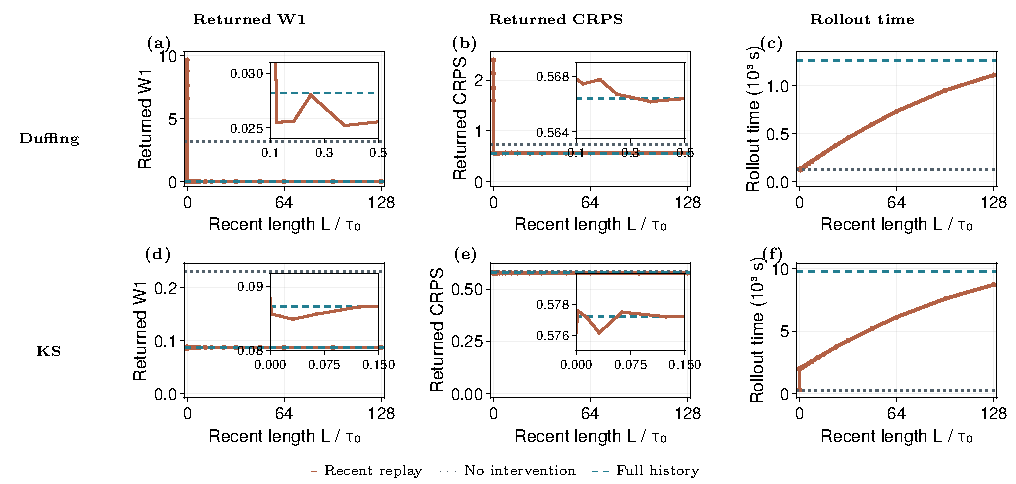
\includegraphics[width=\linewidth,height=.68\textheight,keepaspectratio]{figures/figA03.pdf}
\caption{\textbf{Replay length, quality and computation.} Duffing panels (a--c) and KS panels (d--f) show returned W1, CRPS and rollout time for 300 members over $200\tau_0$. Zero length denotes boundary input alone. Insets show $0.1$--$0.5\tau_0$ for Duffing and $0$--$0.15\tau_0$ for KS. Horizontal references show no intervention and full history, whose length grows with time. Axes are linear, with system-specific vertical ranges. Time is in $10^3$ seconds and includes generation and replay/bookkeeping, excluding diagnostics; each policy has one timing.}\label{fig:duffing-replay-cost}
\end{figure}

\subsubsection{Additional ensemble realizations and physical initial conditions}
Three new reservoir banks, trained on the original data with unchanged model settings, are crossed with two new physical initial conditions. All six Duffing combinations improve returned W1, spread loss and CRPS under the original selected scheme (Fig.~\ref{fig:crossed-replication}). W1 reductions range from 99.0\% to 99.3\%, and CRPS reductions from 19.5\% to 29.7\%. One combination required additional reserve training: the original 450-model pool could not complete blind initial refill, whereas a pool of 750 completed it using 212 reserve members. The final ensemble remains at 300. Original model checkpoints are unchanged, and expanding the pool reproduces the previously successful same-bank cohort exactly. This combination is marked separately; its original reserve-budget failure remains recorded. The three banks share the two physical starts, so the six pairs are not six independent draws of both factors. All six KS combinations also improve the three losses: W1 reductions are 62.8--68.0\%, spread-loss reductions 66.7--72.9\% and CRPS reductions 0.84--1.74\%. All KS cohorts complete the original 450-model refill budget. Each system is analyzed separately; the combinations are a targeted consistency check under fixed training data and presets.
\begin{figure}[!htbp]
\centering
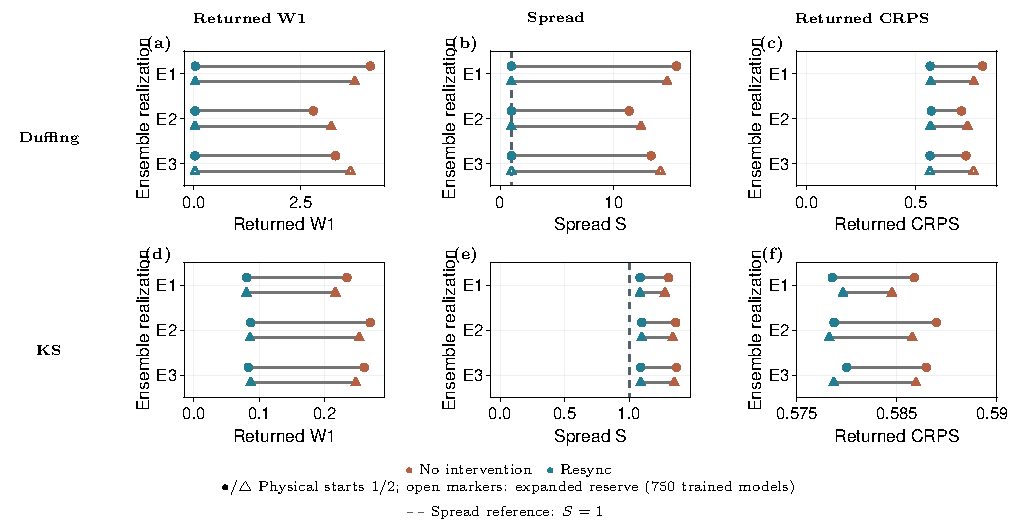
\includegraphics[width=\linewidth,height=.68\textheight,keepaspectratio]{figures/figA04.pdf}
\caption{\textbf{Paired outcomes across ensemble realizations and physical starts.} Duffing panels (a--c) and KS panels (d--f) show returned W1, spread and CRPS. E1--E3 identify the three independently generated reservoir-model ensembles. Circles and triangles distinguish the two physical starts; horizontal lines connect no intervention and Resync for the same ensemble and physical start. Open markers identify the combination requiring a training pool of 750 rather than 450 models; every returned ensemble still contains 300 members. The dashed line marks the spread reference $S=1$. Each point summarizes $200\tau_0$ with 300 members. The KS CRPS axis spans 0.575--0.595 to show the small paired changes. The design is crossed and no independent-run confidence interval is inferred. }\label{fig:crossed-replication}
\end{figure}


All 28 dense-history policies and all six paired ensemble--start combinations are complete for each system. KS own and returned forecasts remain finite, with complete scoring truth; all dense policies share the initial own-output hash and the full-history run reproduces its stored anchor diagnostics. These ensemble-level scores do not estimate sustained member recovery. Recovery persistence and auxiliary-system convergence require dedicated protocols. A recovery assessment would use wholly post-intervention own outputs, predefined distributional and temporal reference ranges, and a prespecified duration without further correction, together with matched no-intervention continuations.


\noappendix
\codedataavailability{The reproducibility record contains source/configuration hashes, case-specific data manifests, model/cohort identifiers, selection histories, calibration summaries and compact test-window tables. It also records the distinct sources used in Figure~\ref{fig:main-population-views} and the postselection analyses. Raw full-forecast trajectories were not retained for every run; validated compact summaries and explicitly scoped replay exports support the reported figures and tables. \textcolor{red}{[Public release: insert repository URLs, persistent identifiers and access conditions.]}}

% Author contributions, competing interests and acknowledgements remain deferred
% at the author's request. See versions/gmd/AUTHOR_CONFIRMATIONS.md before submission.
\bibliographystyle{copernicus}
\bibliography{resync_references,refs_new}
\end{document}
